Estabelecidos os requisitos pretendidos para a
implementação desta fase, verificou-se que seria
necessário realizar algumas adaptações à arquitetura
adotada na fase anterior de forma a cumprir os
novos objetivos.
\newline

\begin{center}
    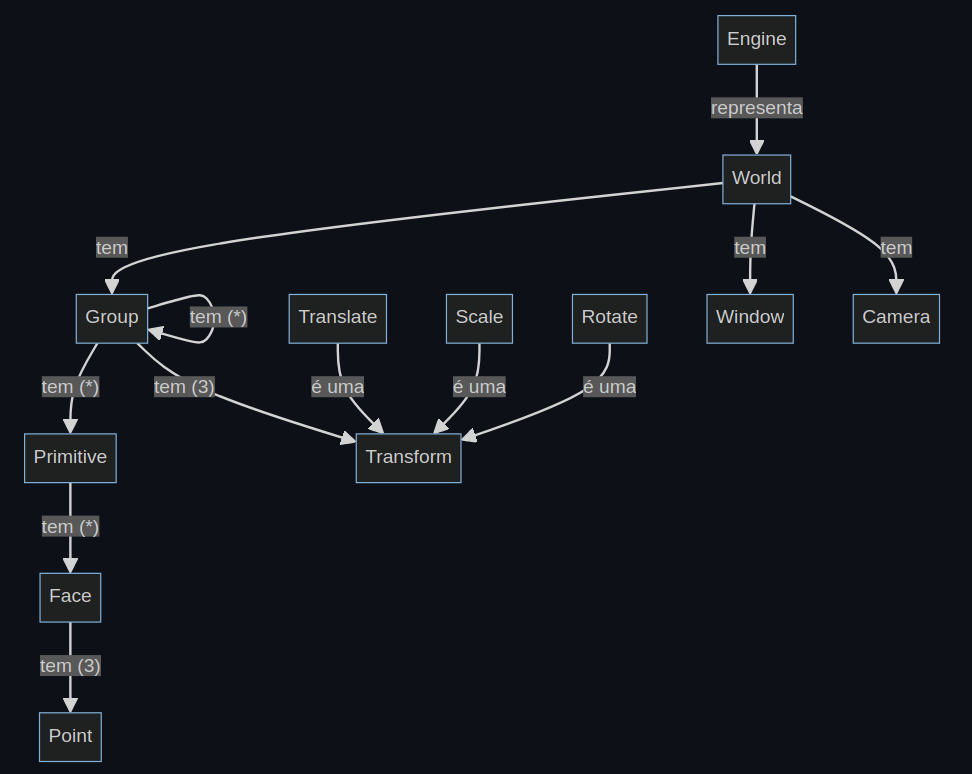
\includegraphics[width=0.8\textwidth]{imgs/concept.png}
    \captionof{figure}{Modelo de Domínio do Motor Gráfico}
    \label{fig:engdom}
\end{center}

\noindent
Aproveitando a semelhança em termos de propriedades das
diversas transformações, decidiu-se seguir uma
estrutura que estabelecesse alguma relação entre elas.
\newline
\break
\noindent
Criou-se, portanto, uma super-classe que estabelecesse
uma definição global focada nestas semelhanças (valores
de aplicação dos eixos, aplicação das transformações em
si, etc...), de forma a puder tirar proveito desta
definição global para a aplicação de transformações
no grupo. Um grupo possui, portanto, um conjunto de
transformações.
\newline
\break
\noindent
Já para a implementação dos sub-grupos, optou-se por
fazer uso da recursividade, uma vez que as propriedades
possíveis dos grupos em si são sempre as mesmas. Esta
recursividade permite, então, a um grupo armazenar um
conjunto de grupos dentro de si.